\documentclass{article}
\usepackage[utf8]{inputenc}
\usepackage{graphicx}
\usepackage{enumerate}
\renewcommand{\baselinestretch}{1.25}
\interfootnotelinepenalty=10000

\title{Final Project Writeup}
\author{Computer Science 51 2021}

\begin{document}

\maketitle

\section{Introduction}
I extended MiniML by adding a lexically scoped evaluator, floats, division, and a greater than symbol. 
\section{Lexical}
To implement the lexically scoped evaluator, I first copied my \textit{eval\_d} function and adjusted it according to the rules for lexical semantics in the textbook. I realized that there were many similarities between \textit{eval\_d} and \textit{eval\_l}, so I decided to abstract away the similarities to avoid unnecessary code reuse and to preserve the edict of irredundancy. \\\\
My original strategy for this was to adjust \textit{eval\_l} so that it only evaluated itself for the cases in which it differed from \textit{eval\_l}, and otherwise simply called \textit{eval\_d}. However, I realized that this might not preserve the edict of intention.\\\\ I therefore decided to create a functor which, after being passed in a specific type of evaluation, would evaluate it accordingly. Therefore, the specific implementation of \textit{eval\_d} and \textit{eval\_l} are behind the abstraction barrier, and the edict of intention is preserved: it is clear to users of my code that \textit{eval\_d} and \textit{eval\_l} are different. However, the functor abstracts away their similarities to preserve the edict of irredundancy. \\\\
To demonstrate this extension, simply call \textit{./miniml.byte} and run the repl. My repl outputs the substitution, dynamic, and lexical evaluations, so it is easy to see how \textit{eval\_l} and \textit{eval\_d} differ by inputting an expression that will have a different output in each evaluator.
\subsection{Differences Between Lexical and Dynamic Evaluations}
There are various conditions in which the evaluator returns a different result under the different semantics. I walk through and demonstrate a few examples of this below.\\
\begin{enumerate}[A.]
\item
In this example, we first set $x$ equal to 2 in a function $f$ where we take a $y$ and output an $x*y$, and then set $x$ equal to 1 before calling the function on 21. In the lexical semantics, the $x$ in the definition of $f$ refers to outer $x$, which is of course 2. However, in the dynamic semantics, the $x$ in the definition of $f$ refers to the most recent $x$, and is therefore 1. Therefore, the different cases return different results.\\As the substitution semantics are lexically scoped, they return the same result as the lexical semantics.
\begin{figure}[h]\begin{center}
    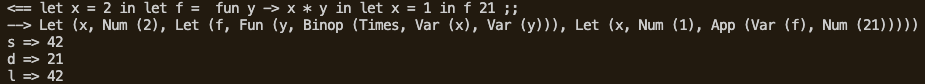
\includegraphics[width =\textwidth]{lddiff1.png}
    \caption{Semantics Example A}
\end{center} \end{figure}
\item
In this example, we first set $x$ equal to 10 in a function $f$ where we take a $y$ and output another function, which takes a $z$ and outputs a $z*(x+y)$, then calling $f$ on 11 and 2. \\\\
When we apply $f$ to 11, we return a function from $z$ to $z*(x+y)$. However, we return this out of the context in which $y$ is defined. Therefore, the dynamic semantics will return an \textit{unbound variable} error, while the lexical and substitution semantics will handle it just fine.
\begin{figure}[h]\begin{center}
    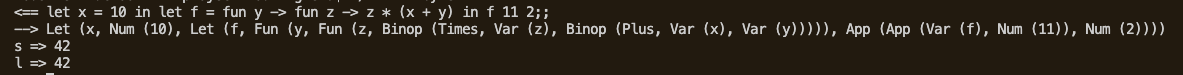
\includegraphics[width =\textwidth]{lddiff2a.png}
    \caption{Semantics Example B1}
\end{center} \end{figure}\\
Here I have set the evaluator to only use dynamic semantics, returning an \textit{unbound variable} error.
\begin{figure}[h]\begin{center}
    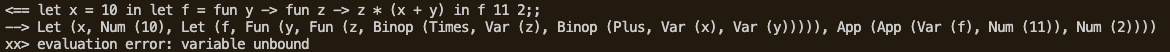
\includegraphics[width =\textwidth]{lddiff2b.png}
    \caption{Semantics Example B2}
\end{center} \end{figure}
\item We can correct or repair this error by ensuring that $y$ has a binding before the function $f$ is called. Here dynamic semantics still return something different than lexical and substitution semantics, but is able to handle this 2-argument function. Dynamic semantics will take the function as if it is being applied to 12 and 2 instead of 11 and 2, because it uses the environment in which y is equal to 12 as opposed to 11.

\begin{figure}[h]\begin{center}
    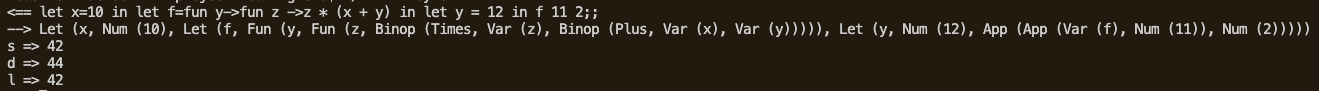
\includegraphics[width =\textwidth]{lddiff3.png}
    \caption{Semantics Example C}
\end{center} \end{figure}

\item In this next example, we set $x$ equal to 2 in a function $f$ where we take a $y$ and output the sum of $x$ and $y$, then setting $x$ equal to 8 and calling $f$ on $x$. \\\\
In the dynamic semantics, when we set $x$ equal to 8, we override the $x$ in the body of the function. Therefore, when we call $f$ on $x$ and therefore set $y$ equal to $x$, we return $8+8$ or 16. In lexical and substitution semantics, however, we maintain the original binding of $x$ to 2, therefore returning $2+8$ or 10.
\begin{figure}[h]\begin{center}
    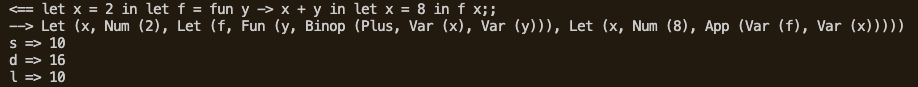
\includegraphics[width =\textwidth]{lddiff4.png}
    \caption{Semantics Example D1}
\end{center} \end{figure}
\\
If we never set $x$ equal to 8, however, then all three semantics will return the same result, as they have the same values for $x$.
\begin{figure}[h]\begin{center}
    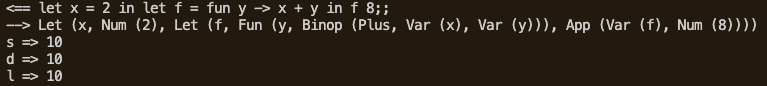
\includegraphics[width =\textwidth]{lddiff4a.png}
    \caption{Semantics Example D2}
\end{center} \end{figure}
\item
In this last example, we set $x$ equal to 1 in a function $f$ where we take a $y$ and output the sum of $x$ and $y$, then setting $x$ equal to 2 and calling $f$ on $3$. \\\\
In the dynamic semantics, when we set $x$ equal to 2, we override the $x$ in the body of the function. Therefore, when we call $f$ on $3$ and therefore set $y$ equal to $3$, we return $2+3$ or 5. In lexical and substitution semantics, however, we maintain the original binding of $1$ to 2, therefore returning $1+4$ or 4.
\begin{figure}[h]\begin{center}
    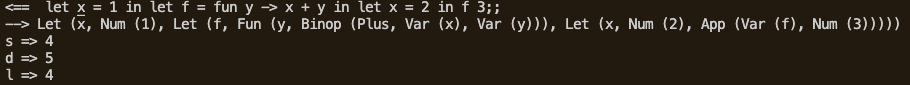
\includegraphics[width =\textwidth]{lddiff5.png}
    \caption{Semantics Example E}
\end{center} \end{figure}
\end{enumerate}

\section{Float}
I added the atomic type of \textit{float} to the language. I did this by updating the type of \textit{expr} to include \textit{Float}, augmenting all \textit{binop} and \textit{unop} evaluators to account for float arithmetic, and extending the MiniML lexer and parser to account for floats. \\\\
I decided that the lexer and parser would take symbols of +  $ -$ $   {\sim}-$   *   / for both integers and floats, and that the evaluator would then convert those to  +. $-.$ ${\sim}-.$ *. /. if they were attached to a float. I did this for ease of use for the user.\\I raise an error if the user attempts to add, subtract, multiply, or divide different types.
Here is an example of my repl evaluating a float:\\
\begin{figure}[h]\begin{center}
    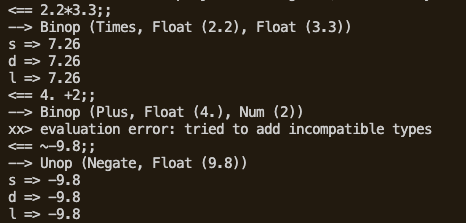
\includegraphics[width =0.8\textwidth]{Float.png}
    \caption{Float Examples}
\end{center} \end{figure}

\section{Greater Than}
I added the symbol $>$ to the language. I did this by updating the type of \textit{binop} to include \textit{GreaterThan}, augmenting all \textit{binop} evaluators to account for float arithmetic, and extending the MiniML lexer and parser to understand $>$ as greater than.\\I raise an error if the user decides to compare an integer to a float or vice versa. \\
Here is an example of my repl evaluating a GreaterThan:
\begin{figure}[h]\begin{center}
    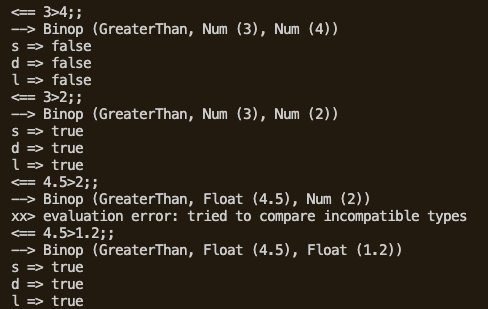
\includegraphics[width =0.8\textwidth]{greaterthan.png}
    \caption{Greater Than Examples}
\end{center} \end{figure}
\\\\\
\section{Division}
I added the symbol $/$ for division to the language. I did this by updating the type of \textit{binop} to include \textit{Divide}, augmenting all \textit{binop} evaluators to account for division, and extending the MiniML lexer and parser to understand $/$ as division. \\\\ I raise an error if the user attempts to divide a zero or divide an integer by a float (or vice versa).\\\\
Here is an example of my repl evaluating a Divide:\\
\begin{figure}[h]\begin{center}
    \includegraphics[width =0.6\textwidth]{divideint.png}
    \caption{Integer Division Examples}
\end{center} \end{figure}
\begin{figure}[h]\begin{center}
    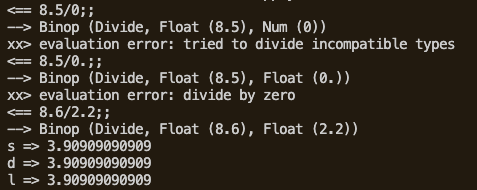
\includegraphics[width =0.75\textwidth]{dividefloat.png}
    \caption{Float Division Examples}
\end{center}\end{figure}

\end{document}
